\documentclass[10pt]{article}
\usepackage{enumerate}
\usepackage{tikz,tikz-cd,tikz-3dplot,pgfplots}
\usepackage{amsmath,amsthm,amssymb,amsfonts,amsthm}
\usepackage{mathrsfs}
\usepackage{bm,bbm}
\usepackage{braket}
\usepackage{slashed}
\usepackage{tensor}
\usepackage{indentfirst}
\usepackage[a4paper, total={6.5in, 9in}]{geometry}
\usetikzlibrary{decorations.markings,positioning,decorations.pathmorphing}
\allowdisplaybreaks
\pgfplotsset{width=10cm, compat=1.16}
\renewcommand\bra[1]{{\langle{#1}|}}
\renewcommand\ket[1]{{|{#1}\rangle}}
\renewcommand\bfdefault{b}

\newtheorem{theorem}{Theorem}[section]
\newtheorem{lemma}[theorem]{Lemma}
\newtheorem{corollary}{Corollary}[theorem]
\theoremstyle{definition}
\newtheorem{definition}{Definition}[section]
\theoremstyle{remark}
\newtheorem{remark}{Remark}[section]

\DeclareMathOperator{\sech}{sech}
\DeclareMathOperator{\csch}{csch}
\DeclareMathOperator{\arcsec}{arcsec}
\DeclareMathOperator{\arccot}{arccot}
\DeclareMathOperator{\arccsc}{arccsc}
\DeclareMathOperator{\arccosh}{arccosh}
\DeclareMathOperator{\arcsinh}{arcsinh}
\DeclareMathOperator{\arctanh}{arctanh}
\DeclareMathOperator{\arcsech}{arcsech}
\DeclareMathOperator{\arccsch}{arccsch}
\DeclareMathOperator{\arccoth}{arccoth} 

\begin{document}
	metric convention: $(+,-,-,-)$
	
	Lagrangian:
	\[\mathcal{L}=\frac{1}{2}\partial_{\mu}\phi\partial^{\mu}\phi-\frac{1}{2}M^{2}\phi^{2}+\partial_{\mu}\chi^{\dagger}\partial^{\mu}\chi-g\phi\chi^{\dagger}\chi.\]
	
	\section{Diagram 1}
	\begin{center}
		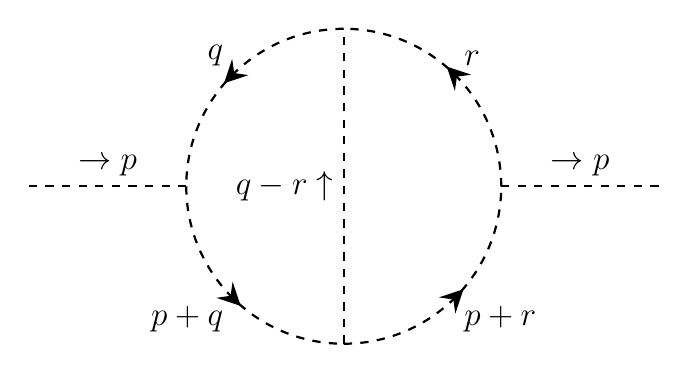
\begin{tikzpicture}[thick,decoration={markings,mark=at position 0.5 with {\arrow[scale=2]{stealth[sep=-0.75mm]}}}]
			\tikzstyle{every node}=[font=\large]
			\def\len{2cm}
			\draw[dashed] (-2*\len,0) -- (-\len,0);
			\draw[dashed] (2*\len,0) -- (\len,0);
			\draw[dashed,postaction={decorate}] (\len,0) arc (0:90:\len);
			\draw[dashed,postaction={decorate}] (0,\len) arc (90:180:\len);
			\draw[dashed,postaction={decorate}] (-\len,0) arc (180:270:\len);
			\draw[dashed,postaction={decorate}] (0,-\len) arc (270:360:\len);
			\draw[dashed] (0,-\len) -- (0,\len);
			\node at (-1.5*\len,0) [above] {$\rightarrow p$};
			\node at (1.5*\len,0) [above] {$\rightarrow p$};
			\node at (-0.7*\len,-0.7*\len) [below left] {$p+q$};
			\node at (-0.7*\len,0.7*\len) [above left] {$q$};
			\node at (0,0) [left] {$q-r\uparrow$};
			\node at (0.7*\len,-0.7*\len) [below right] {$p+r$};
			\node at (0.7*\len,0.7*\len) [above right] {$r$};
		\end{tikzpicture}
	\end{center}
	\[\Pi_{1}(p^{2})=g^{4}\int\frac{d^{d}q}{(2\pi)^{d}}\frac{d^{d}r}{(2\pi)^{d}}\frac{1}{q^{2}}\frac{1}{(p+q)^{2}}\frac{1}{r^{2}}\frac{1}{(p+r)^{2}}\frac{1}{(q-r)^{2}-M^{2}}.\]
	We first deal with the $r$-integral:
	\begin{align*}
		I_{1}&:=\int\frac{d^{d}r}{(2\pi)^{d}}\frac{1}{r^{2}}\frac{1}{(p+r)^{2}}\frac{1}{(q-r)^{2}-M^{2}}\\
		&=2\int\frac{d^{d}r}{(2\pi)^{d}}\int_{0}^{1}dx\,\int_{0}^{1-x}dy\frac{1}{[(1-x-y)r^{2}+y(p+r)^{2}+x((q-r)^{2}-M^{2})]^{3}}\\
		&=2\int\frac{d^{d}r}{(2\pi)^{d}}\int_{0}^{1}dx\,\int_{0}^{1-x}dy\frac{1}{(r'^{2}-\Delta_{r})^{3}}\\
		&=\frac{-i\Gamma(3-\frac{d}{2})}{(4\pi)^{d/2}}\int_{0}^{1}dx\,\int_{0}^{1-x}dy\frac{1}{\Delta_{r}^{3-d/2}},
	\end{align*}
	where $r'=r-xq+yp$ and $\Delta_{r}=-x(1-x)q^{2}-y(1-y)p^{2}-2xyqp+xM^{2}$.
	Now the total integral becomes
	\[\Pi_{1}(p^{2})=g^{4}\frac{-i\Gamma(3-\frac{d}{2})}{(4\pi)^{d/2}}\int_{0}^{1}dx\,\int_{0}^{1-x}dy\int\frac{d^{d}q}{(2\pi)^{d}}\frac{1}{q^{2}}\frac{1}{(p+q)^{2}}\frac{1}{\Delta_{r}^{3-d/2}}.\]
	Let's look at the $q$-integral:
	\begin{align*}
		I_{2}&:=\int\frac{d^{d}q}{(2\pi)^{d}}\frac{1}{q^{2}}\frac{1}{(p+q)^{2}}\frac{1}{\Delta_{r}^{3-d/2}}\\
		&=\frac{\Gamma(7-\frac{d}{2})}{\Gamma(3-\frac{d}{2})}\int_{0}^{1}dz\int_{0}^{1-z}dw\int\frac{d^{d}q}{(2\pi)^{d}}\frac{z^{2-d/2}w(1-z-w)}{[z\Delta_{r}+w(p+q)^{2}+(1-z-w)q^{2}]^{7-d/2}}.
	\end{align*}
	The denominator is
	\begin{align*}
		D&:=z\Delta_{r}+w(p+q)^{2}+(1-z-w)q^{2}\\
		&=(1-z-xz+x^{2}z)q^{2}+(-yz+y^{2}z+w)p^{2}+2(-xyz+w)pq+xzM^{2}\\
		&=(1-z-xz+x^{2}z)\left(q+\frac{-xyz+w}{1-z-xz+x^{2}z}p\right)^{2}+\left(-\frac{(-xyz+w)^{2}}{1-z-xz+x^{2}z}-yz+y^{2}z+w\right)p^{2}+xzM^{2}\\
		&=:(1-z-xz+x^{2}z)q'^{2}-\Delta_{q}.
	\end{align*}
	Then
	\[\int\frac{d^{d}q}{(2\pi)^{d}}\frac{1}{[(1-z-xz+x^{2}z)q'^{2}-\Delta_{q}]^{7-d/2}}=\frac{-i(-1)^{-d/2}}{(4\pi)^{d/2}}\frac{\Gamma(7-d)}{\Gamma(7-\frac{d}{2})}\frac{1}{(1-z-xz+x^{2}z)^{d/2}}\frac{1}{\Delta_{q}^{7-d}}.\]
	Bringing all together,
	\[\Pi_{1}(p^{2})=g^{4}\frac{-(-1)^{-d/2}}{(4\pi)^{d}}\Gamma(7-d)\int_{0}^{1}dx\int_{0}^{1-x}dy\int_{0}^{1}dz\int_{0}^{1-z}dw\frac{z^{2-d/2}w(1-z-w)}{(1-z-xz+x^{2}z)^{d/2}}\frac{1}{\Delta_{q}^{7-d}}.\]
\end{document}